\chapter{Principy a historie regulárních výrazů}\label{sec:Principle}

Abychom mohli porozumět, jakým problémem se v této práci vlastně zabýváme, tak si musíme zadefinovat co jsou
regulární výrazy, jak fungují a jak se jednotlivé implementace mohu lišit. Následovně si vysvětlíme, jak lze zjednodušit
pochopení těchto výrazů, popřípadě jak rychle najít chybu ve vlastním výrazu. 

Předtím než si vysvětlíme blíže jak fungují samotné regulární výrazy, je potřeba si první objasnit význam několika pojmů z teoretické informatiky\footnote{vědní obor na pomezí mezi informatikou a matematikou}.

\section{Formální jazyk}
Formální jazyk je libovolná množina koečných slov nad určitou abecedou. 
Slova chápeme jako retězece znaků, která jsou příjimaná zadaným jazykem.
Tato slova musí být sice konečná ale množina těchto slov může být nekonečná. 
Tyto jazyky mohou být definovány regulárními výrazy, formální gramatikou,
konečnými automaty a dalšími. Regulární jazyky jsou tak jednou z možných definic formálních jazyků.

\section{Konečný automat}
Ve spojení s regulárními výrazy se často pojí konečné automaty, jedná se o další oblast v teoretické informatice.
Proto abychom pochopili proč je tato oblast pro nás důležitá, musíme si vysvětlit co vlastně jsou.

Konečný automat je model jednoduchého počítače, který má určitý počet stavů a přechodů \cite{Havrlant}. 

Stavy jsou typycky zakreslovány jako kružnice, a každý automat musí obstahovat alespoň jeden počáteční stav,
ale může jich také obsahovat více. To samé platí pro konečný/é stav/y. Konečné stavy se vyznačují jako kruh z dvojtou čárou a počáteční stavy jsou, 
označovány jako stav do kterého vede šipka, která ale nevychází z jiného stavu.
Prechody jsou pak šipky vedoucí z jednoho stavu do druhého, jsou označeny přechodovým symbolem.
Tyto šipky nám říkají že pokud chceme přejít z jednoho stavu do druhého, tak musíme v příjimaném slově se posunout o
daný symbol. Pokud to není možné, tak nemůžeme přejít do tohoto stavu.

Tyto automaty dělíme na deterministické a nedeterministické, zkráceně DKA (deterministický konečný automat) a NKA (nedeterministický konečný automat).
DKA mohou mít v daném stavů pro každý znak abecedy \textbf{maximálně} jeden přechod, dále \textbf{nemohou obsahovat tzv. prázný znak} často označovaný řeckým písmenem epsilon $\epsilon$.
NKA naopak obojí umožňují, prázné znaky nám umožňují změnu stavu bez změny aktuální pozice v hledaném slově. 
Každý NKA lze převést na ekvivalentní DKA.

\begin{figure}[!h]
	\centering
	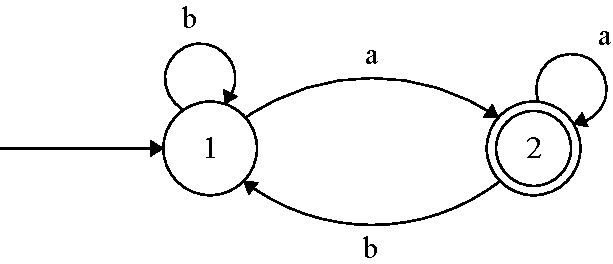
\includegraphics[width=0.6\textwidth]{Figures/DFA_example.pdf}
	\caption{Příklad deterministického automatu příjamjící slova obsahující písmena z abecedy \{a, b\} končící písmenem a}
	\label{fig:DFAex}
\end{figure}

\begin{figure}[!h]
	\centering
	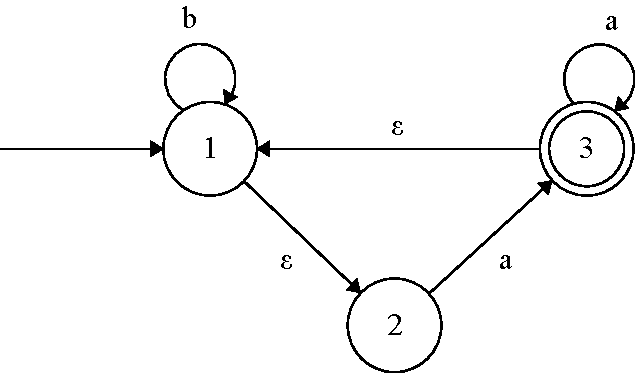
\includegraphics[width=0.6\textwidth]{Figures/NFA_example.pdf}
	\caption{Příklad nedeterministického automatu ekvivalentního k předchozímu deterministickému}
	\label{fig:NFAex}
\end{figure}

\section{Původ, vznik a implementace}
Regulární výrazy byly poprvé nadefinovány Americkým matematikem \textbf{Stephan Cole Kleene}, jako regulární jazyky. 
Dále se aplikovali v teoretické informatice, jako podkategorie \textbf{teorie automatů} a součást \textbf{formálních jazyků}.
Ačkoliv byli nadefinovány začátkem padesátých let, tak jejich využití v počítačích nastalo až na konci šedesátých let a to v 
jedním z nejznámějších operačních systémů UNIX.

\subsection*{Thompsonovo sestrojení}

\textbf{Ken Thompson} byl člověkem kdo navrhnul první implementaci převodu ragulárního výrazu na NKA využívanou v počítačích, která se používá do dnes. 
Algoritmus se pojmenoval \textbf{Thompson's construction} (Thompsonovo sestrojení), který převádí textovou reprezentaci výrazu na ekvivalentní nedeterministický automat.
Toto sestrojení je využito v této práci, proto si musíme vysvětlit jak funguje.

Používá se často implementace NKA, jelikož je poměrně jednoduchá na implementaci a
také dovoluje oproti DKA využití zpětného krokování (backtracking) a rozhlédnutí se kolem sebe (lookaround).
DKA mají výhodu že jsou rychlejší oproti NKA, ale jsou typycky větší než jejich ekvivalentní NKA a neumožňují již zmíněné funkce. 
Někdy se ale využívá například kombinace DKA i NKA, kdy DKA kvůli vyšší rychlosti se použije na vyhledání daného slova a pokud bylo nalezeno, 
tak se využije NKA pro jejich rozšířené možnosti.

Výsledný NKA má právě jeden vstupní a výstupní stav. Aby došlo ke správnému sestrojení NKA z Regulárního výrazu, musíme se řídit několika pravidly, pro ukázku si pár těchto pravidel ukážeme.

Prázdný výraz \textit{$\epsilon$}, je převedený na vstupní stav přechod \textit{$\epsilon$} a konečný stav.
\begin{figure}[!h]
	\centering
	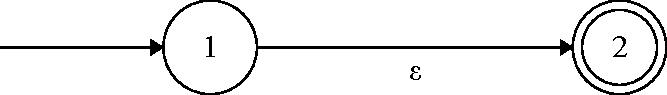
\includegraphics[width=0.6\textwidth]{Figures/NFA_epsilon.pdf}
	\caption{Převedený prázný výraz \textbf{$\epsilon$}}
	\label{fig:NFAepsilon}
\end{figure}

Výraz \textit{a}, je převedený podobně jako prázdný výraz, ale s rozdílem přechodu \textit{a} místo \textit{$\epsilon$}.
\begin{figure}[!h]
	\centering
	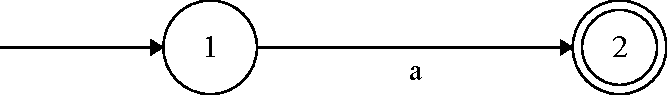
\includegraphics[width=0.6\textwidth]{Figures/NFA_a.pdf}
	\caption{Převedený výraz \textbf{a}}
	\label{fig:NFAa}
\end{figure}

Pro zadaný výraz \textbf{s|t}, kdy \textit{s} je levá strana varianty a \textit{t} je pravá strana varianty, platí že ze stavu \textit{q} vedou dva přechody
\textit{$\epsilon$} na počáteční stavy variant \textit{s} a \textit{t}. Z těchto počátečních stavů dále pokračuje sekvence stavů \textit{N(s)} pro \textit{s} a \textit{N(t)} pro \textit{t}.
Konce variant \textit{s} a \textit{t} mají jediný přechod \textit{$\epsilon$} na konečný stav.
\begin{figure}[!h]
	\centering
	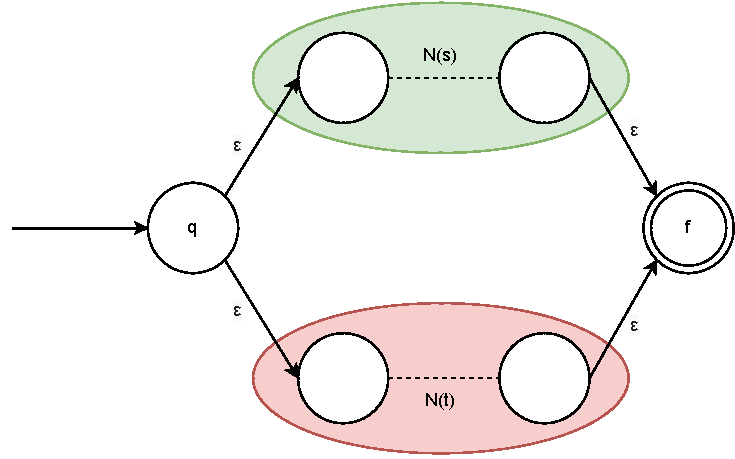
\includegraphics[width=0.8\textwidth]{Figures/NFA_union.pdf}
	\caption{Převedený výraz \textbf{s|t}}
	\label{fig:NFAunion}
\end{figure}

Další pravidla pro sestrojení lze například najít na anglické wikipedia stránce pro thompsonovo sestrojení \cite{Wikipedia_2023}.